% !TeX encoding = UTF-8
% !TeX spellcheck = es_ES
% !TeX root = ../ComponentCatalog.tex
%!TEX root=../ComponentCatalog.tex

\begin{table}[H]
    \centering
    \renewcommand\theadfont{\bfseries}
    \setlength{\tabcolsep}{10pt}
    \renewcommand{\arraystretch}{1.5}

    \begin{tabular}{|c|c|c|c|c|c|}
        \hline
        \multicolumn{6}{|c|}{\thead[b]{Botones TH Amazon}} \\
        \hline
        \thead[b]{Nota} & \multicolumn{5}{|l|}{STD = 6x6x3}\\ \hline
        \multicolumn{6}{|c|}{
            \begin{tikzpicture}[baseline=0]
                \begin{scope}
                    \clip (0,0) rectangle (13,6);
                    \node[inner sep=0pt] at (6.5,4)
                        {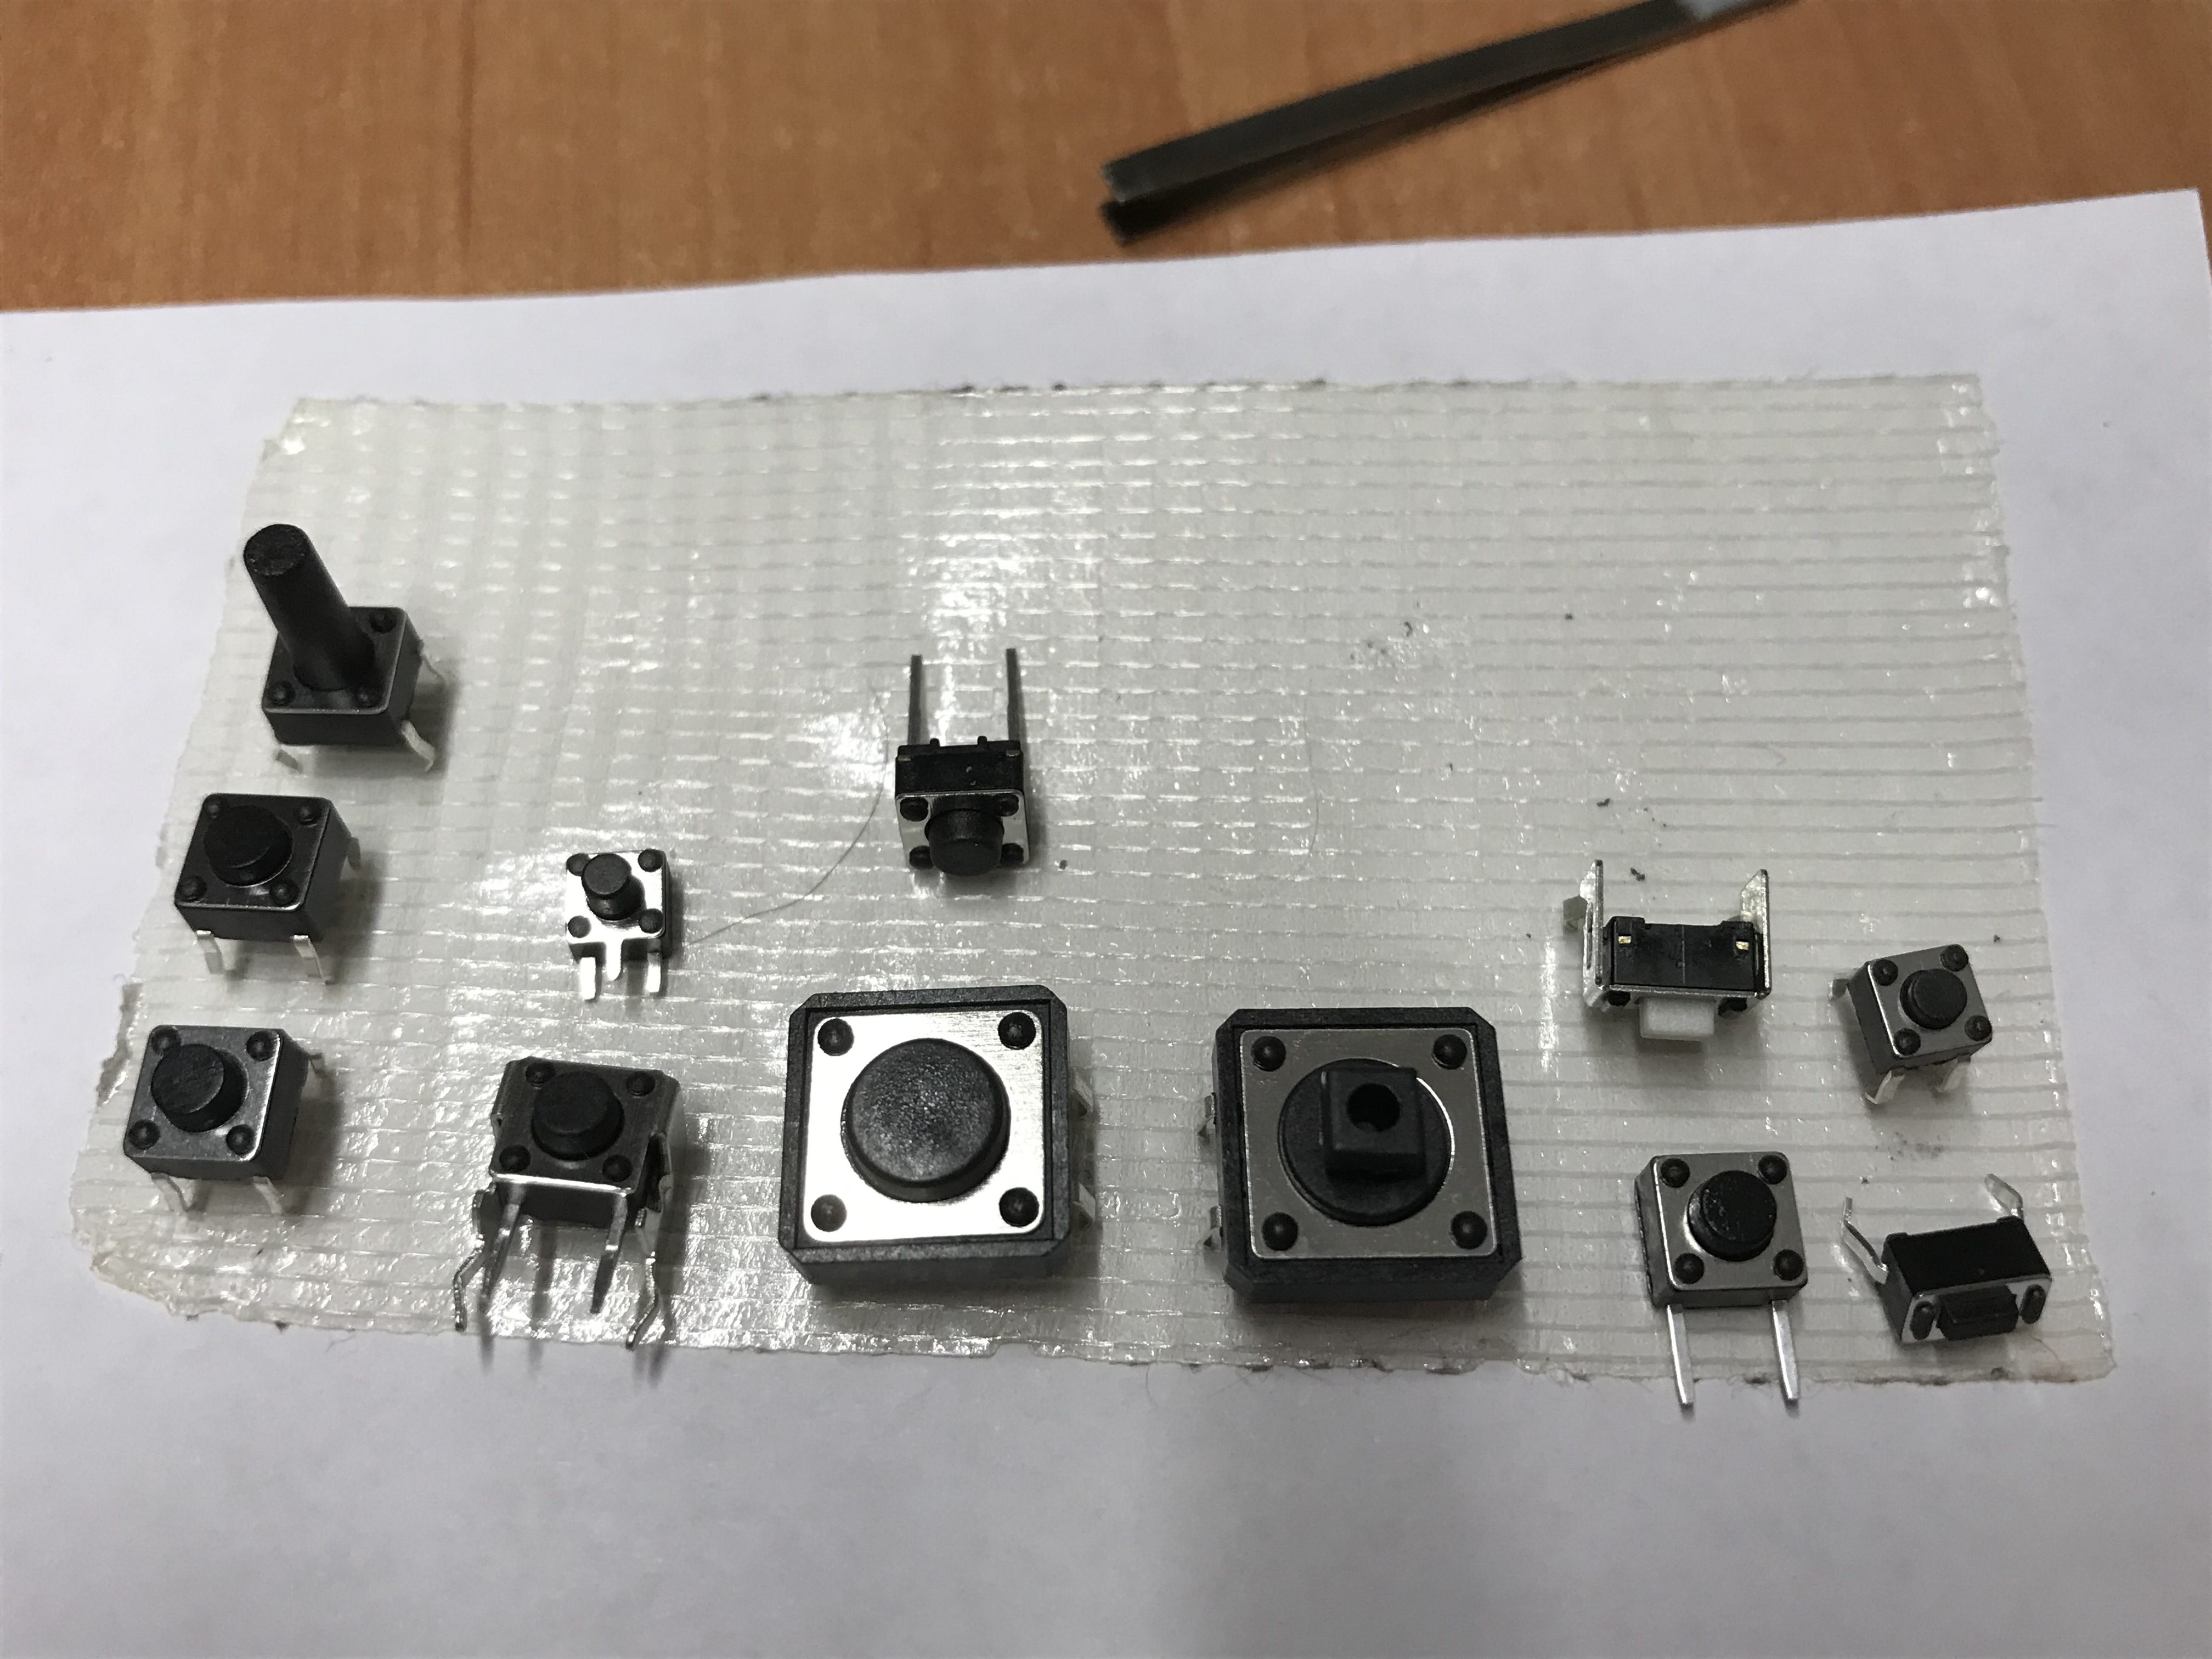
\includegraphics[scale=.1]{pictures/thBtn.jpg}};
                \end{scope}
                \addvmargin{1mm}
            \end{tikzpicture} 
        } \\
        \hline

        STD (BL)&  &\multirow{2}{*}{STD (PL)} & &  & \\ \cline{1 - 2} \cline{4 - 6}
        STD (BN)& 4.3x3x4.3 & & & 7.2x3x3.5 &4.5x4.5x2.7 \\ \hline
        STD (BP)& STD' (L)  &12x12x3 &12x12x3 & STD (L) &6x3.3x3 \\ \hline

        \thead[b]{Uso} & \multicolumn{5}{|l|}{Tener Catalogo Botones para buscar}\\ \hline
        \thead[b]{Ubicacion} & \multicolumn{5}{|l|}{Terraza}\\ \hline

    \end{tabular}
    \caption{Botones SMD Amazon}
    \label{tab:BtnThAmazon}
\end{table}


